\section{Tasks, Projects and Activities}
\subsection{Organization}
In fact, Sylvain Hunault and I needed to prepare the web site and trackers in two months. Since Sylvain Hunault knows much more about electronic cards, then he was in charge of the hardware part, including all the antennae, batteries and electronic cards, and I was familiar with ruby on rails because of my experience, so I focused on the software part. Since the web site was much more problematic and needed to be enhanced further, after preparing the hardware part, we two both worked into the web site. Normally we worked separately according to the distributed functions which are necessary to be added into the site. And also we worked together when we needed to integrate all the unitary functions, or when we were in front of some problems. We shared our knowledge and information obtained, and discussed together. In addition, all the useful information and our source code were put into the Github (a tool of the distributed revision control and source code management) repertoire.


Actually, the development of website was function-oriented, the branch "master" was the principal branch which would be released to the public, besides every one or two weeks, a new branch was created, which means a new feature was released. Before merging every new branch into the "master" branch, all unitary tests and integrate tests should be passed. 
\begin{figure}[h!]
    \centering
    \includegraphics[width=12cm]{allbranches.png}
    \caption{All function-oriented branches }
    \label{fig-sample}
\end{figure}

%============ new features
\subsection{New features}
%============ New style and New Home Page
\subsubsection{New style and New GUI}
%\begin{figure}[h!]
%    \centering
%    \includegraphics[width=20cm]{oldversion.png}
%    \caption{old version GUI }
%    \label{fig-sample}
%\end{figure}

The web site created for the WRSC 2014 (project SWARMON) contains a no open sources CSS and Layout(left image in the figure before), and at the beginning of 2015, the web site was updated with the latest CSS3 which is open sources and more beautiful and customizable(right image in the figure before). Our current web site based on the latest CSS3.

\begin{figure}[h!]
\centering
\includegraphics[width=14cm]{oldversion.png}
\caption{Old home page, WRSC2014(left), MYR2015(right) }
\label{fig-sample}
\end{figure}

\begin{figure}[h!]
\centering
\includegraphics[width=13cm]{homepage.png}
\caption{New Home Page }
\end{figure}

%====== add team#show
\begin{figure}[h!]
\centering
\includegraphics[width=8cm]{oldteamshow.png}
\caption{old team show}
\label{fig-sample}
\end{figure}
In the previous version, the web site could only display the basic information about every team, like: team name, leader, members and description. In order to simplify the access of pages and the use for users, we add two fields to show the team's members and robots by loading with two Ajax(asynchronous JavaScript and XML) requests to permit the easy management for members and robots.



%====== add robot#show
Similar to the page team\#show, the previous web site could only display the basic information about every robot, like: name, owner(team), category. These information are essential but insufficient, especially for the new users, who are not familiar with our web site. For example, they do not know if they had registered to participate a mission (if they want to know, they need to go to the page attempts, and check if their robot name in the whole list one by one and also if they want to know the time for missions, or/and the time for every attempt, they need to go another page to check all the information). So in order to facilitate the use of web site, we decided to put all these information into the page robot\#show. Also we had thought a lot about the form to display all these information to users. Since the logic is that a robot participates several missions, and for every mission, there could be more attempts, and every score and tracker id were attached to an unique attempt. So based on this hierarchical order, it will be better to choose a tree structure chart to show the logic. In order to meet our need, we had chosen google org(organization) charts which are open source and all APIs are provided and published by Google company freely. Since our web site was built up by ruby on rails, and google org charts were released as JavaScript APIs, from this, every time when the site loads the robot\#show page, it will recall an Ajax request and send all the associated information from the ruby part to the JavaScript part, then in the JavaScript part, we could use the org charts' APIs directly. 
\begin{figure}[h!]
\centering
\includegraphics[width=15cm]{orgcharts.png}
\caption{Google org charts example }
\label{fig-sample}
\end{figure}

%============== Sortable \& Searchable Table
\subsubsection{Sortable \& Searchable Table}

The previous version web site(WRSC 2014 in Galway) used the form of table to list all the information for teams, robots, missions, members and etc. And all these tables were only sortable by the alphabetic order.
\begin{figure}[h!]
\centering
\includegraphics[width=15cm]{newtable.png}
\caption{Comparison of two type tables, UP is the previous version, DOWN is the current version}
\label{fig-sample}
\end{figure}
The only sortable table works well when there is not enormous data, if we suppose that there are more than 100 members in our database, and if you want to find the information about one member and you had only the name of this member, it will be stupid to check the whole list just by eyes. Furthermore, if the web site displays more than 10 records in one page, which often makes the user feel uncomfortable and inefficient. Based on these reasons, we choose a flexible and customizable JavaScript plug-in "DataTable". DataTable is very simple to use as a jQuery plug-in with a huge range of customizable options, and the functions which we are interested in most are sorting(which makes the table sortable by alphabetic order), filtering (which makes the table searchable, we can search one element by typing part of the keyword) and pagination (which limits the number of elements in one page, also it will make the page loading be faster and reduce the pressure of server because of the limitation of elements in the page). What's more, "DataTable" provides more APIs which also make the html table flexible, the developers are easy to get the index or element in the table just by calling the functions, comparing to the static html table, the "DataTable" is more dynamic and interacted for users.

\subsubsection{Improved Account Management}
\begin{enumerate}
\item{\textbf{Sign UP}}
\begin{figure}[h!]
\centering
\includegraphics[width=12cm]{signup.png}
\caption{Comparison of page Sign Up }
\label{fig-sample}
\end{figure}

The new sign up page add three new features:
\begin{itemize}
\item{\textbf{Uploading local image file instead of typing a link}}


In the old version web site, the user could only typing an image file url to upload the logo. And at the side of server, it adopts a gem called "fastimage", which could handle of the url and get the image from this url, but one limitation is the image size could not larger than several hundred pixels * several hundred pixels, as a matter of fact, this size is quite small comparing to the normal image file which is nearly several mega bytes. So for this reason, the logo field is nearly useless because of the inconvenient. 


In order to solve this problem, in the new web site, we used a gem called "carrierwave"(an open source free project, all the codes are available in their Github repertoire), which permits to upload whatever format file. Furthermore, here we need to treat the image file, so at the side of rails application, it requires another gem "mini\_magick"(Unlike RMagick, MiniMagick is a much thinner wrapper around ImageMagick, that's why we choose MiniMagick rather than RMagick), at the side of server machine, it requires the software "ImageMagick" (under Linux, type "convert -v" to check if the "ImageMagick" was installed).


Once all the gems are installed successfully, a new folder "uploaders" will be added into Rails.root(the root path of rails application)/app, and the creation of uploading action is similar to create a controller/model in rails application, either by the command "rails generate uploader nameoffile", or by create the file manually. And then in the model, we need to mount the uploader, in our case, we need to add:  
\begin{lstlisting}
"mount_uploader :logo, MemberlogoUploader" 
\end{lstlisting}
in the file Rails.root/app/models/member.rb. 


After that, the attribute "logo" of "member" would only accept a file uploader object, even at the beginning, we define the type of logo is a string. If we dive deep into the database(either look through by rails console, or by SQLite database browser, the attribute "logo" is filled by a complicated object where it contains the original file name which means the name of uploaded image file, also the name of full name which means the uploaded image file's absolute file name--path in the rails application + file name, and other information). Due to this reason, once an image file was uploaded, we should not change the position of this file, because in the database, the image file was just saved as the path and the name rather than the image self.


What's more, "carrierwave" provided some other customizable convenient options, for instance, we can define our own store directory to put all the image files. Actually by default, all the files accessible for any other user should be put into Rails.root/public. Also do not trust the file uploaded via internet, we should make sure all the files in public directory were inexecutable. From this, "carrierwave" also provide an option to set the extension white list, where we can limit the file format to avoid the virus. In addition, if the rails application was launched by a Linux machine, we can set the permission of the directory "public" to make sure all the users except the owner(admin) could only read and write, but not execute. One way possible to do so is by using the command 
\begin{lstlisting}
chmod 766 <directory>
\end{lstlisting}
Then with the command 
\begin{lstlisting}
ls -l
\end{lstlisting}
we can check if the directory permission is
\begin{lstlisting}
drwxrw-rw-
\end{lstlisting}

Also we can define different versions of image files with different sizes based on the initial image, which will be applied once the image file is uploaded.

\item{\textbf{Simple captcha}}


Another important change for the sign up page is that we added the captcha to filtering human user and avoid basic attacks. The realization of captcha is also simple. We used a gem called "simple\_capthca2"(an open sources free project, all the codes are also available from Github repertoire). 
As controller Based, we just need to do:
Add the following line in the file “app/controllers/application.rb”
\begin{lstlisting}
ApplicationController < ActionController::Base
  include SimpleCaptcha::ControllerHelpers
end
\end{lstlisting}

In the view file within the form tags add this code
\begin{lstlisting}
<%= show_simple_captcha %>
\end{lstlisting}

and in the controller's action authenticate it as
\begin{lstlisting}[language=Ruby]
if simple_captcha_valid?
  do this
else
  do that
end
\end{lstlisting}

\item{\textbf{Activate by email}}


In the new web site, we also added the function of sending emails to activate the new account when one user registers on the site. As we did not have any specific email account, we choosed Gmail account as our admin email account because of several reasons.
\begin{itemize}
\item In order to display the google map in our web site, we register a google account to obtain a google map JavaScript API key, so already even we did not choose Gmail as our main email, we should at least use the google account for JavaScript API.
\item Gmail service is free and easy to use, although Google limits the amount of mail a user can send, via its portable SMTP server, and the amount of sending emails is limited 99 per day, regarding our web site focuses on the participators, even maybe there are some other users, 99 is already enough for the email function. In addition, if we want much more capacity, if the budget allows, we could buy the service of Gmail SMTP server in the future.
\item Gmail is secure, wide used and compatible with others email service provider. And sometimes, Gmail is too secure to use. And the problem we meet at the beginning is that we had sent an email by configuring the SMTP server in our Rails Application, then Google detected this operation was done by machine not a web user and our email was blocked. In order to solve these types of problems, we need to configure our Gmail to less secure status by going to this page https://www.google.com/settings/security/lesssecureapps and changing to less secure.
\end{itemize}
When the Gmail account was setted correctly, and also we can send emails to other users, another problem came to our views. How can we send a unique link to the user and also how can we identify this link is associated with the relative user ? Actually before creating a user, we create a new activate token(which is used to send to the user) and a activate digest(which is saved into database and used to identify the relative user). 
In the file Rails.root/app/models/member.rb
\begin{lstlisting}
	before_create :create_activation_digest
	def create_activation_digest
		self.activation_token  = Member.new_token
		self.activation_digest = Member.digest(activation_token)
	end
\end{lstlisting}
In fact, all the passwords, or more generally, the important information are encrypted before saving into the database by using the popular gem "Bcrypt". Obviously the security of encryption depends on the longer of generated token(Here we used 64 bits to generate a random token, normally it is long enough) and the algorithm(In this case, it is "Eksblowfish"--"expensive key schedule Blowfish", which based on the algorithm Blowfish. Cryptotheoretically, this is no stronger than the standard Blowfish key schedule). Also we need to pass the user's email address as an argument in the url, then we can identify the token with the associated member which was saved in the database found by the email address.
In the file Rails.root/app/models/member.rb
\begin{lstlisting}
    def Member.digest(string)
   		cost = ActiveModel::SecurePassword.min_cost ? 
   			   BCrypt::Engine::MIN_COST : BCrypt::Engine.cost
		BCrypt::Password.create(string, cost: cost)
    end
    
    def Member.new_token
   	 	SecureRandom.urlsafe_base64
   	end
\end{lstlisting}
Then the creation of email sending is just like any other page, firstly create the controller with desired actions, and then create the views which would be sent to the user later.
\end{itemize}

\item{\textbf{Sign in}}

\begin{figure}[h!]
\centering
\includegraphics[width=10cm]{signin.png}
\caption{Comparison of page Sign In }
\label{fig-sample}
\end{figure}

In the new sign in page, we had also added two new features:
\begin{itemize}
\item{\textbf{Remember the User}}


The function of "Remember me" is quite similar to sending the activation link to users. If the user choose to remember in the computer, then the server would write the user id and a remember token into cookies. With the function cookies.signed which provided by rails application, the contents in the cookies would be encrypted. Furthermore, something should be noticed: 
\begin{itemize}
\item Cookies exist in different browsers in the same computer, so if the user has more than one browser (for instance: one Firefox and one Chrome), the cookies will be shared between the two browsers. 
\item The contents in the cookies contains two values, one is what we want to save into the cookie, and the other one is the expire date which indicates the validate time for the cookie. If we use "session", which contains the same contents as cookies, but the expire date is from when the contents were created to when the user close the browser.
\end{itemize} 

\item{\textbf{Reset the Password}}


"Reset the password" has the similar principle as the activation email sending. When a user request to reset its password, it needs to provide its email address as a reference. Then the server generate a token and a digest, send the link which contains the user's email address and a reset token to the user. After, when the user clicked the link, the server verifies the digest with the token, if it is the correct token, then the user could change its information.
\end{itemize}

\end{enumerate}

\subsubsection{Admin Markers Creation}
\begin{itemize}
\item{Markers}


The pages of real-time and replay worked well last year, but the markers(the buoys) were not added to these pages, also the web site did not display any marker information, which was inconvenient for the observers following the traces of robots. Inspired by these objectives, we designed to add an administration tool to add markers to a specific mission. Based on the initial designed schema by Bastien DROUOT and Benoit BOURDON, finally we obtained the new function of adding markers for administrators.
\begin{figure}[h!]
\centering
\includegraphics[width=15cm]{designedadminmarkers.png}
\caption{designed admin markers }
\label{fig-sample}
\end{figure}

\begin{figure}[h!]
\centering
\includegraphics[width=15cm]{adminmarkers.png}
\caption{admin markers }
\label{fig-sample}
\end{figure}
The realization of creation of markers based on the Google map JavaScript APIs provided by Google company(https://developers.google.com/maps/documentation/javascript/markers). Actually, the JavaScript APIs provided the possibilities to add point, line, polygon and circle into the google map. And for each type markers, there are two possibilities to draw on the map: either draw the marker with the given coordinates, so then the marker is fixed on the map and can not be modified later, or draw the marker by clicking on the map directly, then it is up to the developer to add the options to drag or to move the marker or even change the size of marker dynamically. 
As a matter of fact, the last version could display some markers in the robots' path by using a gem called "gmaps4rails" which is easy to be applied into rails application, but since this gem also based on the Google map JavaScript API, in addition the gem changed and limited some options from Google APIs, so we could not use all the functions provided by Google API via the gem. In order to get more freedom, we had abandoned the gem, furthermore, the google API provided more customizable options(for example, we can change the icon of marker, add some animations for displaying the marker, the possibility to hide the marker instead of deleting the whole marker and also the adapt zoom for all the markers).
\begin{figure}[h!]
\centering
\includegraphics[width=15cm]{examplemarkers.png}
\caption{admin markers }
\label{fig-sample}
\end{figure}
\item{InfoWindow}
Moreover, Google map JavaScript API offers the possibilities to add some events to the marker or even some events for the mouse motion. Among all these options, what we are interested most is the possibility to display the infowindow for every marker to specify the accurate and precise coordinates of the robot's position. In fact, there are two ways to achieve the requirements.
\begin{itemize}
\item{Google API}
As a matter of fact, Google API provides the possibility to show the coordinate when clicking on the map directly, because google map capture the mouse action on the google map and then print the coordinates directly, but the limitation is that google map could only displays the coordinates of markers, if the user want to know much more information about the team(like: team name, the id of attempt and the tracker id), Google API could not meet all these demands. One advantage is that using google API do not need to communicate the server, so the response will be faster and it will reduce the pressure of server.
\begin{figure}[h!]
\centering
\includegraphics[width=15cm]{ajaxinfowindow.png}
\caption{admin markers }
\label{fig-sample}
\end{figure}
\item{Ajax request to communicate with server}
Obviously, communicating with server, we could get all the information we want, but the problem is that we need to send the Ajax requests, which will cost much more time, especially in most cases, there are hundreds and thousands data to display, even if the number of markers is 10 times less than the number of coordinates, we could imagine that 1000 positions need to display, then 1/10 of positions(which means 100) need to show the infowindow, also it means 100 Ajax requests, if every Ajax request lasts 30ms, then 100 Ajax requests last 3s, it means one user click a button one time, it will cost 3s to calculate for the server, when there are more than 10 users do the same things at the same time, the server would be broken absolutely.
\begin{figure}[h!]
\centering
\includegraphics[width=15cm]{apiinfowindow.png}
\caption{admin markers }
\label{fig-sample}
\end{figure}
\end{itemize}
So actually, there is not any better way to do it, the different method meets different requirements, finally we had mixed these two ways to achieve our target.
\end{itemize}

\subsubsection{Auto Scoring and Ranking}
\begin{enumerate}
\item{Scoring}


The WRSC contains 4 missions: Station Keeping, Area Scanning, Triangular Course and Fleet Race. And I was in charge of the scoring for Station Keeping and Area Scanning. So I will introduce the algorithms I had chosen to calculate the score.
\begin{itemize}
\item{Station Keeping}
\begin{itemize}
\item{Description of mission}
As the WRSC rules described, the objective of the station keeping contest is to evaluate controlled sailing in a limited region with time constraints. Each boat must start outside a 45 m x 45 m box, marked by four buoys. In the team slot time, the boat must enter the box. The boat shall leave the box at a time as close as possible to 5 minutes after entering the box. Boats fulfilling the entry and exit criteria are awarded points based on the following formula:
P = max (0, 10 - |Tenter + 300 - Tleave|/10)
Where: Tenter is the timestamp when the boat first enters the box and Tleave is the timestamp
when the boat first leaves the box. If the boat enters and leaves the box several times, any leave timestamps within ten seconds from Tenter are ignored. All timestamps are given in seconds.
\end{itemize}
\item{Area Scanning}
\begin{itemize}
\item{Description of mission}
The course will be divided into 10x10 square sections, each with a width of about 31 m. The sections will be indexed as (i, j), where i goes from 0 to 9 starting at south and going north, and j goes from 0 to 9 starting at west and going east. From the time the boat enters the first section and within a time of 90 minutes, the boat shall pass through as many square sections as possible. The score for the area scanning contest will be calculated as:
P = Npassed/10
where Npassed is the number of entered sections.
The score will be multiplied with a factor determined from oceanographic measurements provided for each visited section. Depth (m), water temperature (\textcelsius), air temperature (\textcelsius), water salinity (\%), conductivity (S/cm), chlorophyll (ug/l), ammonium (mg/l), nitrate (mg/l), chloride (mg/l) and total dissolved solids (mg/l) can be provided. Inclusion of depth data will add 0.2 to the multiplication factor, the other measurements each add 0.1. The multiplication factor is 1.0 initially, and the maximum that can be achieved is 1.5. Each team shall provide data on the team’s performance to the Race Committee within 5 hours after the start of their slot time. The data shall be in XML, specified by the schema below. The data will contain the team name. For each entered square section the section’s indices are required along with a UTC timestamp and corresponding coordinates using <gml:pos> property in WGS-84 (EPSG:4326). Optionally the oceanographic data can be added. Each entered section shall be added only once to the XML data.
\item{algorithm for Area Scanning}
Actually, for the contest area scanning, the Race Committee decided to do the scoring by themselves, but they ask us to verify the GPS data submitted by the teams with XML format with data gathered by our trackers. Fortunately, Åland University of Applied Sciences(ÅUAS) had a python program which can analyse the submitted XML file and then generate a JSON file(which contains all the useful data and this file is easy to be handled by ruby on rails). And then I based on this JSON file, compare the data with the correspondent tracker's data to check if the gaps of positions were under the tolerance. In order to accomplish this task, several steps were adopted:
\begin{enumerate}
\item The participated team should uploading their XML file to their robot's page

(robot\#IdOfTheirRobot). And also I added a time stamp to record the time when the team submitted their XML file because the team should upload their XML file in 5 hours since they had finished their attempts.
\item With python program(provided by Conny Ljunggren, ÅUAS), I need to generate a JSON file manually. Also I had looked into the python program, in fact the python program used a module called "xml.etree.ElementTree", the key point of this program is using this module to analyse XML file. Unfortunately, I did not find any similar module in Ruby to analyse the XML file, but it was also feasible in ruby. It was just like a compilation project, the code source is XML file, and then the target file is JSON file, so then if we define the grammar of XML, define the lexer and Backus Normal Form(BNF), from the Backus Normal Form(BNF), create the parser to analyse the code source, and store all the separate data in the node of Abstract Syntax Tree(AST), then either by using the visitor pattern, or mix erb with visitor pattern, we can generate the target code finally. Since we did not have so much more time, I did not realize this function.
\item Based on the JSON file, ruby could import the JSON file directly, then I can compare the GPS data to the data in our web site and calculate the difference between the two sets of data. Because all the unities of GPS data are in degree, which are incomprehensible for humans, then I transfer the unity in degree to the unity in meter by using the algorithm proposed by this site: 
http://www.movable-type.co.uk/scripts/latlong.html

\begin{figure}[h!]
    \centering
    \includegraphics[width=12cm]{distanceformula.png}
    \caption{latitude longitude to meter formula from Internet}
    \label{fig-sample}
\end{figure}
And also I had tried the official contest's buoys positions. In fact, the Race Committee declared officially the distance between two buoys is about 31m [(60.1050,19.9500);(60.1080,19.9500)], and from the formula, I obtain the distance is a little more than 30m, so the gap is less than 1m which is acceptable by the GPS precision.
\item After the comparison, in ruby there are three possibilities(JSON/YAML/XML) to display the result, finally I choose XML not only to keep coherent with what they submitted, but also easy to read for users. As a matter of fact, files are also like any other resource in the web site(like views), according to the path in the rails application, we can visit the file by typing the url Rails.root/FilePath.
\end{enumerate}
 
\end{itemize}
\end{itemize} 
\item{Ranking}
\begin{itemize}
\item{Improved Model}
The previous version do not contain the function of scoring and ranking, so the old model do not satisfy the new need. Then we proposed a new model, the principle is every attempt has a unique score, every robot has many attempts, equally every robot has many scores, then we just need to take the best score into account for every robot, at last we compare all the scores for all the robots. So we add a new table Score into the model and add some new attributes to the table Robot.
\begin{figure}[h!]
\centering
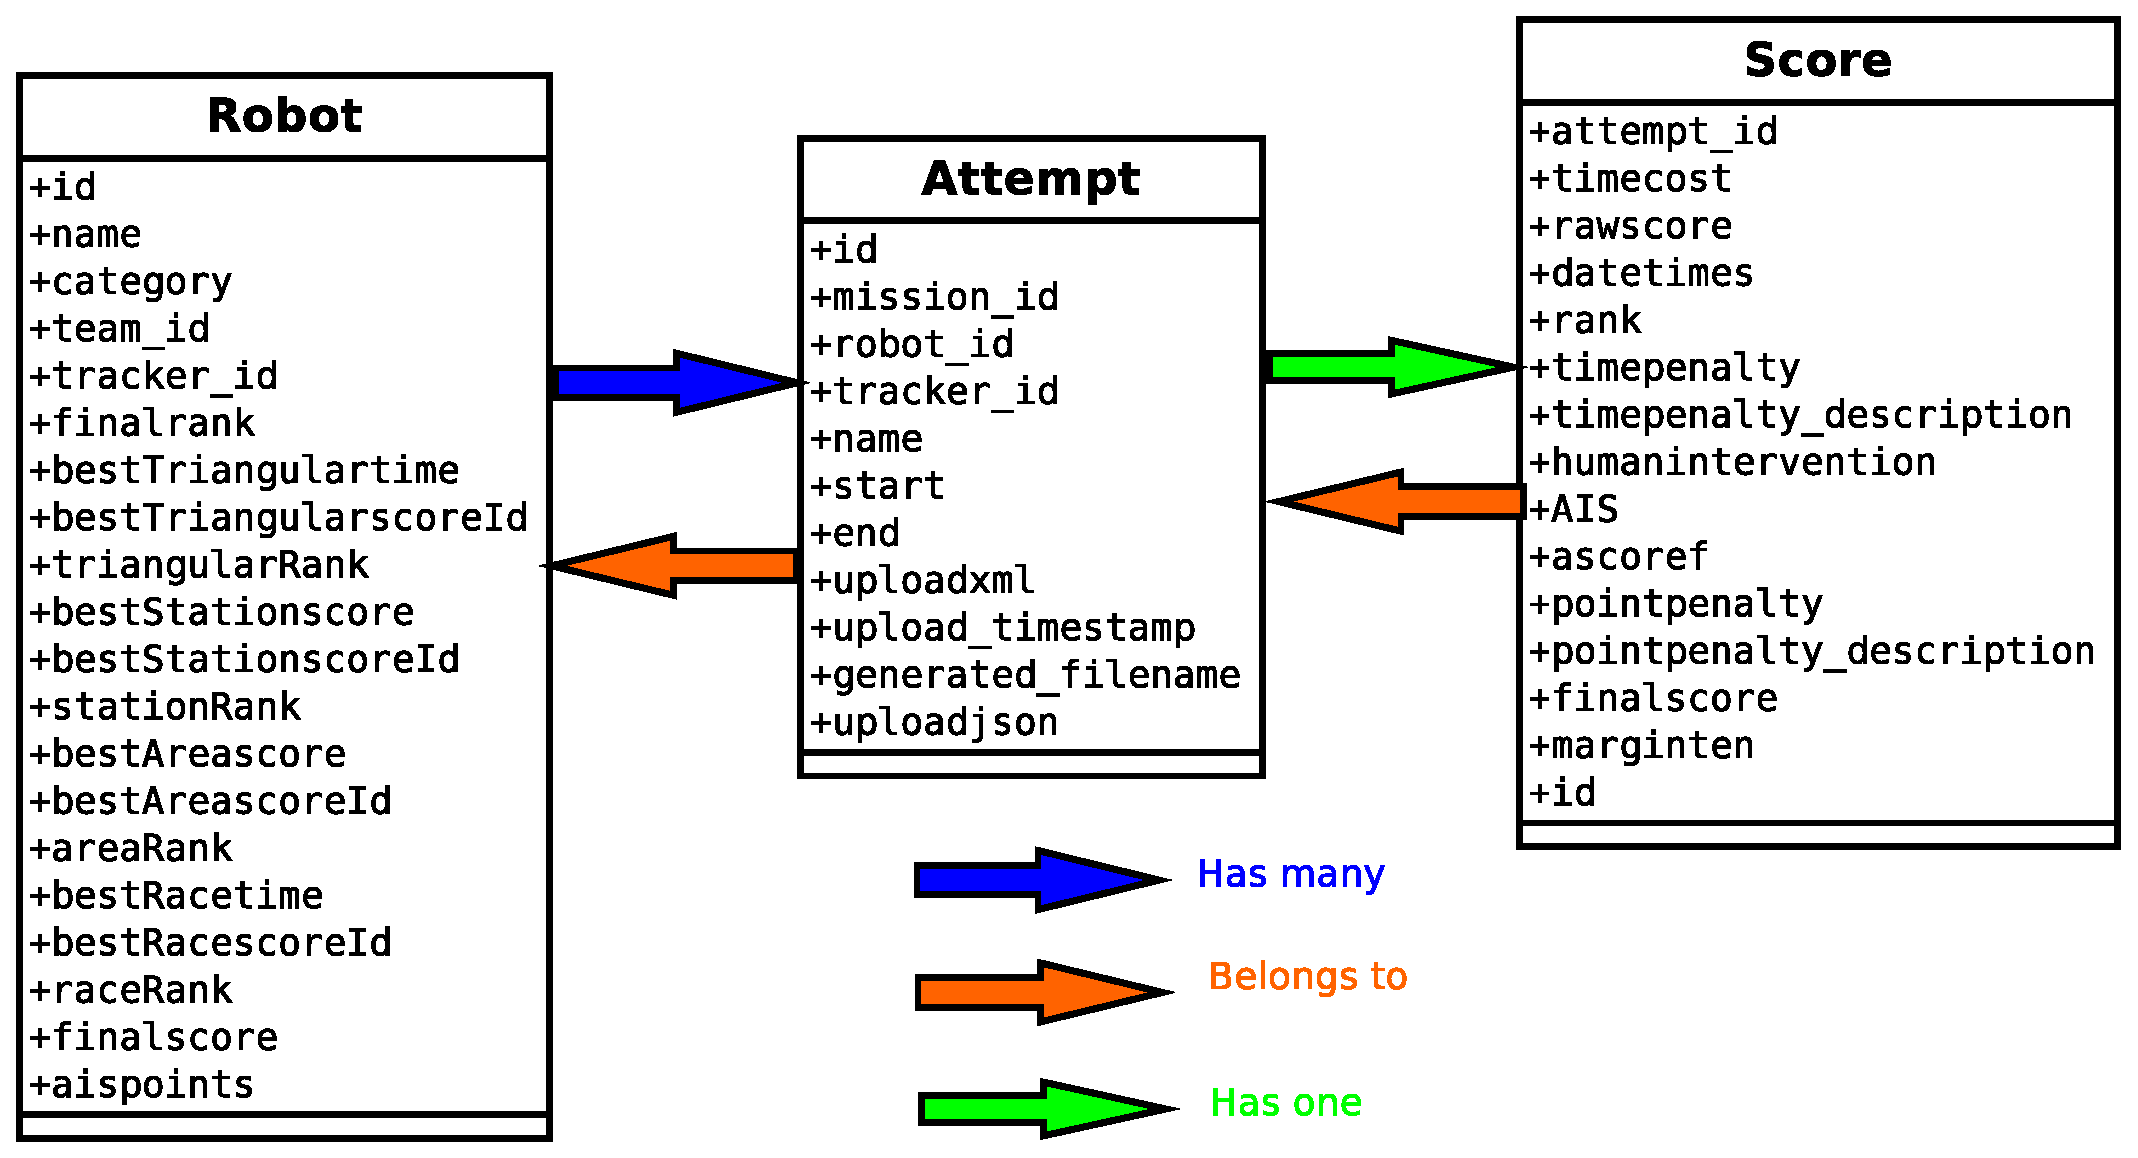
\includegraphics[width=15cm]{improvedpartdatabase.eps}
\caption{new sign in }
\label{fig-sample}
\end{figure}
\item{processes of ranking}
Actually, there are 4 missions for the whole championship, and every mission has different rules and penalties, but the processes of every mission works similarly, when a team finished an attempt, we should create a score for this attempt, from the algorithm we used, we could get the time cost or a raw score differed from missions. Here I take an example of triangular course to illustrate the process to obtain the best score, where Hi means human intervention:
\begin{figure}[h!]
\centering
\includegraphics[width=15cm]{triangular.jpg}
\caption{new sign in }
\label{fig-sample}
\end{figure}
After obtaining the best score for every team, we could calculate the rank. Here something should be noticed, the AIS points are not taken into account in every single mission, but in the final score, we should add the AIS points.


\end{itemize}
\end{enumerate}


Based on all the new features, finally we improved our database which is more complete.
\begin{figure}[h!]
\centering
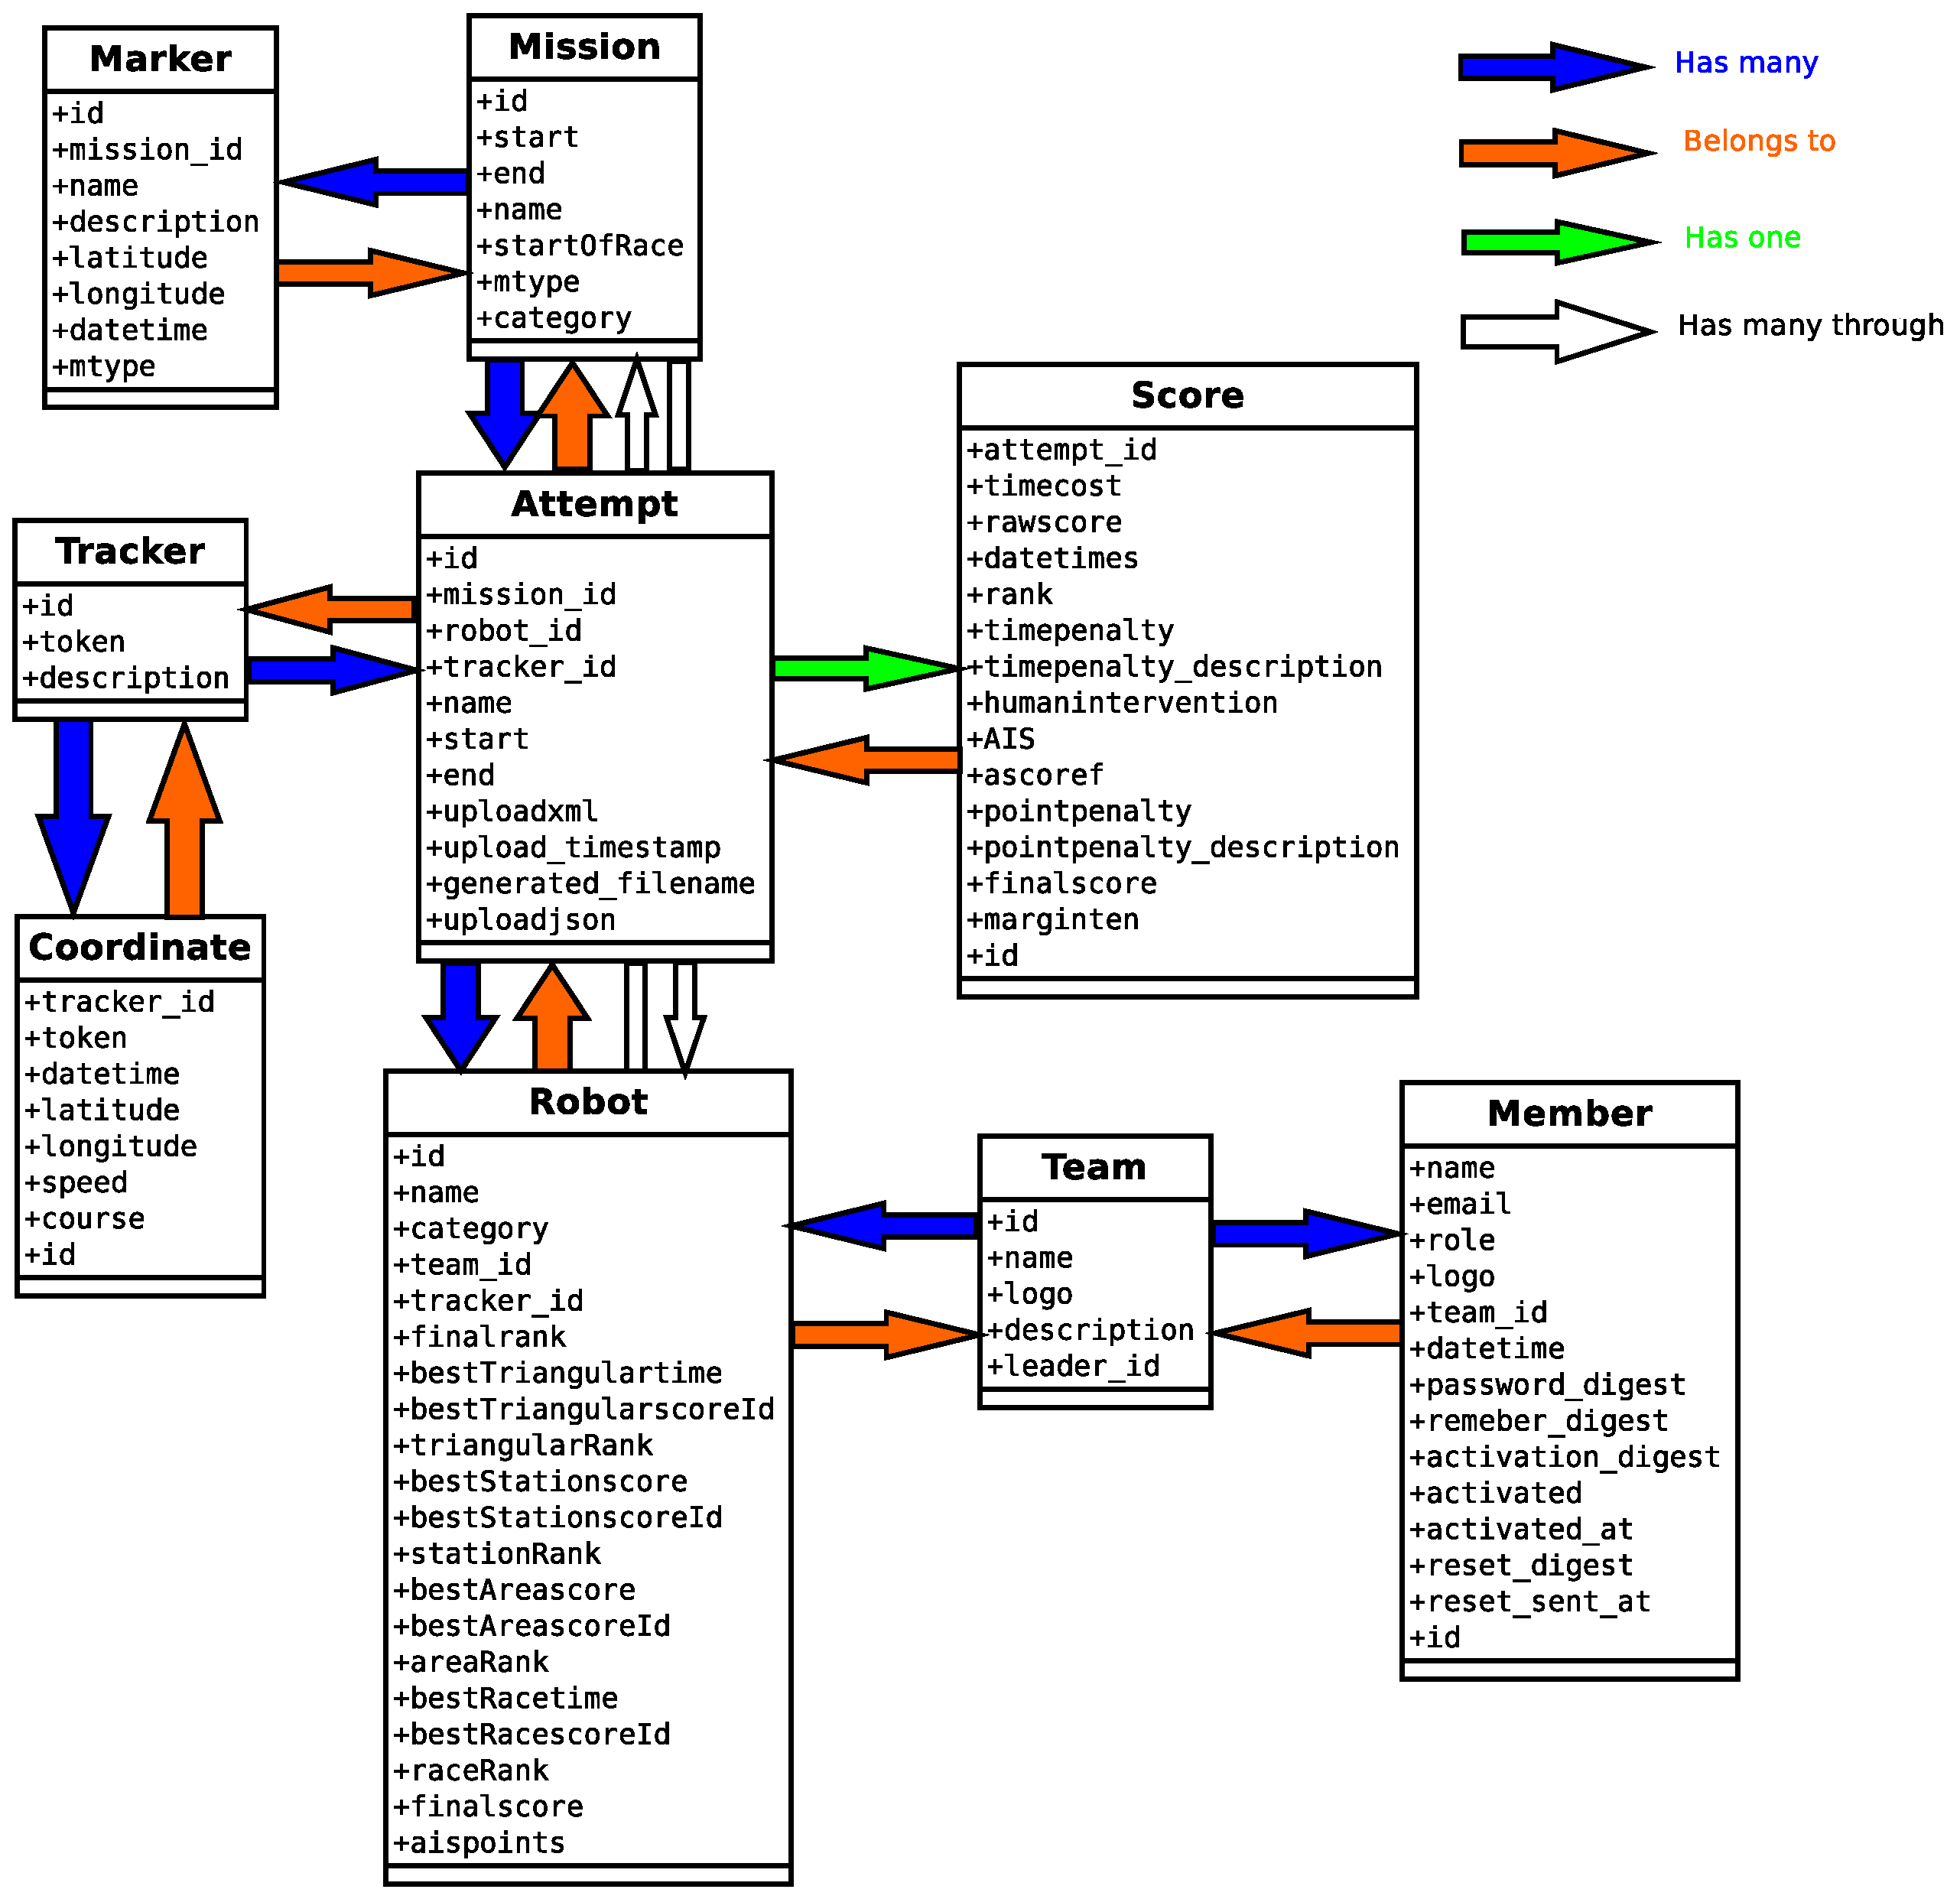
\includegraphics[width=15cm]{database.eps}
\caption{The final Database for WRSC2015}
\label{fig-sample}
\end{figure}
\subsection{Settings in the virtual machine}
After we had finished our development of web site, we need to put our site into the internet. Thanks to Ålcom Mariehamn(A telecommunication company in Mariehamn, Finland) who sponsored a virtual machine to run our server. Initially the server was inaccessible from outside, which means the server do not allow the user from internet to connect to this server. So in order to put our server on the internet, the first thing we need to configure the firewall by using "iptables", since it was a Linux machine. By default, rails application uses the port 3000 to run the server, but then the url will be terminated with :3000, which is not the familiar convention for the most users, so we choose the port 80 rather than the port 3000 to offer our service. 

With the command:
\begin{lstlisting}
sudo iptables -I INPUT -p tcp --dport 80 -j ACCEPT
\end{lstlisting}
we enable the visit outside to the port 80.

After setting the secret\_key\_base into the environmental variable in the virtual machine, we launched the machine with production mode(which is light and safer than development and test mode), our server was well prepared for the service.
\subsection{Result for Tracking System and WRSC}
Fortunately, our web site works quite well, all the functions we added perform as we expected. 
\begin{enumerate}
\item{\textbf{Email}}

Our admin Gmail account works well, it can send the activation emails and reset password emails perfectly, all the users received their emails.
\begin{figure}[h!]
\centering
\includegraphics[width=15cm]{emailrecords.png}
\caption{Admin Gmail sending records}
\label{fig-sample}
\end{figure}

\begin{figure}[h!]
\centering
\includegraphics[width=12cm]{contentemail.png}
\caption{An example of activating email content}
\label{fig-sample}
\end{figure}

\item{\textbf{Tracking system}}


Here are some captures of missions:
\begin{figure}[h!]
\centering
\includegraphics[width=12cm]{resultmissions.png}
\caption{Captures of WRSC mission in the real-time page }
\label{fig-sample}
\end{figure}
As the figures demonstrated, our web site could indicate the whole trace of all robots clearly, the tracking system works perfectly.

\item{\textbf{Scoring and Ranking}}

Before this year, all the scores were given by the Race committee and were measured by humans, but this year, with our tracking system and our algorithms, we can obtain more objective scores, so after discussing with the Race committee, the final result based on our calculations. Here is a quick view of the final standing:
\begin{figure}[h!]
\centering
\includegraphics[width=12cm]{finalranking.png}
\caption{Final Standing of WRSC2015 }
\label{fig-sample}
\end{figure}
Also the uploading file function works well, and based on the submitted data and our trackers' data, here is a hint about the comparison of these two sets of data, finally the maximum difference is about 8 meters which is acceptable.
\begin{figure}[h!]
\centering
\includegraphics[width=8cm]{uploadingfiles.png}
\caption{Uploading file example }
\label{fig-sample}
\end{figure}
\begin{figure}[h!]
\centering
\includegraphics[width=12cm]{xmlfile.png}
\caption{old sign in }
\label{fig-sample}
\end{figure}
\end{enumerate}